\documentclass{beamer}
\usepackage[utf8]{inputenc}

\usetheme{Madrid}
\usecolortheme{default}
\usepackage{amsmath,amssymb,amsfonts,amsthm}
\usepackage{txfonts}
\usepackage{tkz-euclide}
\usepackage{listings}
\usepackage{adjustbox}
\usepackage{array}
\usepackage{tabularx}
\usepackage{gvv}
\usepackage{lmodern}
\usepackage{circuitikz}
\usepackage{tikz}
\usepackage{graphicx}
\usepackage{amsmath}

\setbeamertemplate{page number in head/foot}[totalframenumber]

\usepackage{tcolorbox}
\tcbuselibrary{minted,breakable,xparse,skins}



\definecolor{bg}{gray}{0.95}
\DeclareTCBListing{mintedbox}{O{}m!O{}}{%
  breakable=true,
  listing engine=minted,
  listing only,
  minted language=#2,
  minted style=default,
  minted options={%
    linenos,
    gobble=0,
    breaklines=true,
    breakafter=,,
    fontsize=\small,
    numbersep=8pt,
    #1},
  boxsep=0pt,
  left skip=0pt,
  right skip=0pt,
  left=25pt,
  right=0pt,
  top=3pt,
  bottom=3pt,
  arc=5pt,
  leftrule=0pt,
  rightrule=0pt,
  bottomrule=2pt,
  toprule=2pt,
  colback=bg,
  colframe=orange!70,
  enhanced,
  overlay={%
    \begin{tcbclipinterior}
    \fill[orange!20!white] (frame.south west) rectangle ([xshift=20pt]frame.north west);
    \end{tcbclipinterior}},
  #3,
}
\lstset{
    language=C,
    basicstyle=\ttfamily\small,
    keywordstyle=\color{blue},
    stringstyle=\color{orange},
    commentstyle=\color{green!60!black},
    numbers=left,
    numberstyle=\tiny\color{gray},
    breaklines=true,
    showstringspaces=false,
}


\title 
{4.13.90}
\date{September 25,2025}


\author 
{Abhiram Reddy-AI25BTECH11021}



\begin{document}


\frame{\titlepage}

% Frame: Question
\begin{frame}{Question 4.13.90}
If the distance of the point \( \mathbf{P}(1, -2, 1) \) from the plane 
\[
x + 2y - 2z = \alpha, \quad \text{where } \alpha > 0,
\]
is 5, then the foot of the perpendicular from \( \mathbf{P} \) to the plane is:

\begin{multicols}{4}
\begin{enumerate}
    \item \( \left( \frac{8}{3}, \frac{4}{3}, -\frac{7}{3} \right) \)
    \item \( \left( \frac{4}{3}, -\frac{4}{3}, \frac{1}{3} \right) \)
    \item \( \left( \frac{1}{3}, \frac{2}{3}, \frac{10}{3} \right) \)
    \item \( \left( \frac{2}{3}, -\frac{1}{3}, \frac{5}{2} \right) \)
\end{enumerate}
\end{multicols}
\end{frame}

% Frame: Step 1
\begin{frame}{Step 1: Use Distance Formula}
Let
\[
\mathbf{n} = \begin{bmatrix} 1 \\ 2 \\ -2 \end{bmatrix}, \quad \mathbf{P} = \begin{bmatrix} 1 \\ -2 \\ 1 \end{bmatrix}
\]
The distance from point \( \mathbf{P} \) to the plane is:
\begin{equation}
D = \frac{|\mathbf{n}^T \mathbf{P} - \alpha|}{\|\mathbf{n}\|}
\end{equation}
Compute:
\begin{equation}
\mathbf{n}^T \mathbf{P} = 1 - 4 - 2 = -5
\end{equation}
\begin{equation}
\|\mathbf{n}\| = \sqrt{1^2 + 2^2 + (-2)^2} = \sqrt{9} = 3
\end{equation}
Given \( D = 5 \), solve:
\begin{equation}
5 = \frac{|-5 - \alpha|}{3} \Rightarrow |-5 - \alpha| = 15
\end{equation}
\end{frame}

% Frame: Solve for alpha
\begin{frame}{Step 2: Solve for \(\alpha\)}
From:
\[
|-5 - \alpha| = 15
\]
Case 1:
\begin{equation}
-5 - \alpha = 15 \Rightarrow \alpha = -20 \quad \text{(invalid)}
\end{equation}
Case 2:
\begin{equation}
-5 - \alpha = -15 \Rightarrow \alpha = 10
\end{equation}
So, the plane becomes:
\begin{equation}
x + 2y - 2z = 10
\end{equation}
\end{frame}

% Frame: Foot of perpendicular
\begin{frame}{Step 3: Foot of Perpendicular}
Let the foot be \( \mathbf{Q} = \mathbf{P} + \lambda \mathbf{n} \)

\begin{equation}
\mathbf{Q} = \begin{bmatrix} 1 \\ -2 \\ 1 \end{bmatrix} + \lambda \begin{bmatrix} 1 \\ 2 \\ -2 \end{bmatrix} 
= \begin{bmatrix} 1 + \lambda \\ -2 + 2\lambda \\ 1 - 2\lambda \end{bmatrix}
\end{equation}

Substitute into plane:
\[
(1 + \lambda) + 2(-2 + 2\lambda) - 2(1 - 2\lambda) = 10
\]
\[
1 + \lambda - 4 + 4\lambda - 2 + 4\lambda = 10
\Rightarrow -5 + 9\lambda = 10
\Rightarrow \lambda = \frac{15}{9} = \frac{5}{3}
\]
\end{frame}

% Frame: Final point
\begin{frame}{Step 4: Final Answer}
Substitute \( \lambda = \frac{5}{3} \) into \( \mathbf{Q} \):
\begin{equation}
\mathbf{Q} = \begin{bmatrix} 1 + \frac{5}{3} \\ -2 + \frac{10}{3} \\ 1 - \frac{10}{3} \end{bmatrix}
= \begin{bmatrix} \frac{8}{3} \\ \frac{4}{3} \\ -\frac{7}{3} \end{bmatrix}
\end{equation}

\[
\boxed{
\left( \frac{8}{3}, \frac{4}{3}, -\frac{7}{3} \right)
}
\quad \text{Option 1}
\]
\end{frame}

% Frame: C Code - Function
\begin{frame}[fragile]{C Code – Function}
\begin{lstlisting}[language=C]
#include <math.h>

double distanceFromPointToPlane(double A, double B, double C, double D_plane,
                                double x0, double y0, double z0) {
    double numerator = fabs(A * x0 + B * y0 + C * z0 - D_plane);
    double denominator = sqrt(A * A + B * B + C * C);
    return numerator / denominator;
}
\end{lstlisting}
\end{frame}

% Frame: C Code – Main
\begin{frame}[fragile]{C Code – Main Function}
\begin{lstlisting}[language=C]
#include <stdio.h>

int main() {
    double A = 1, B = 2, C = -2;
    double alpha = 10;
    double x0 = 1, y0 = -2, z0 = 1;
    double distance = distanceFromPointToPlane(A, B, C, alpha, x0, y0, z0);
    printf("Distance from point to plane = %.2f\n", distance);
    return 0;
}
\end{lstlisting}
\end{frame}

% --- FRAME 6: Python Code - Part 1 (Setup) ---
\begin{frame}[fragile]{Python Code: Setup and Locus Data}
    \framesubtitle{Generating Data for the Plot}
    
    We use $c=5$ and an example line with intercepts $a=25/3$ and $b=25/4$.
    
    \lstset{style=PythonStyle}
    \begin{lstlisting}[language=Python]
import numpy as np
import matplotlib.pyplot as plt
from mpl_toolkits.mplot3d import Axes3D

P = np.array([1, -2, 1])
F = np.array([8/3, 4/3, -7/3])
A, B, C, D_plane = 1, 2, -2, 10

fig = plt.figure(figsize=(10, 8))
ax = fig.add_subplot(111, projection='3d')

ax.scatter(*P, color='r', s=100, label=r'Point P(1, -2, 1)')
ax.scatter(*F, color='g', s=100, label=r'Foot of Perpendicular F($\frac{8}{3}, \frac{4}{3}, -\frac{7}{3}$)')

ax.plot([P[0], F[0]], [P[1], F[1]], [P[2], F[2]], 'k--', label='Perpendicular Line PF')

x_min, x_max = -1, 4
y_min, y_max = -4, 4

xx, yy = np.meshgrid(np.linspace(x_min, x_max, 10), np.linspace(y_min, y_max, 10))
    \end{lstlisting}
\end{frame}

% --- FRAME 7: Python Code - Part 2 (Plotting) ---
\begin{frame}[fragile]{Python Code: Plotting the Graphs}
    \framesubtitle{Visualization of the Locus and an Example Line}
    
    \lstset{style=PythonStyle}
    \begin{lstlisting}[language=Python]
zz = (A * xx + B * yy - D_plane) / C

ax.plot_surface(xx, yy, zz, alpha=0.5, rstride=100, cstride=100, color='c')

ax.set_xlabel('X-axis')
ax.set_ylabel('Y-axis')
ax.set_zlabel('Z-axis')
ax.set_title(r'3D Plot of Point, Plane, and Foot of Perpendicular')

ax.legend()
ax.view_init(elev=20, azim=45)
ax.set_box_aspect([np.ptp(a) for a in [ax.get_xlim(), ax.get_ylim(), ax.get_zlim()]]) 

plt.savefig('python_plot.png')
    \end{lstlisting}
\end{frame}

\begin{frame}{Plot}
    \centering
    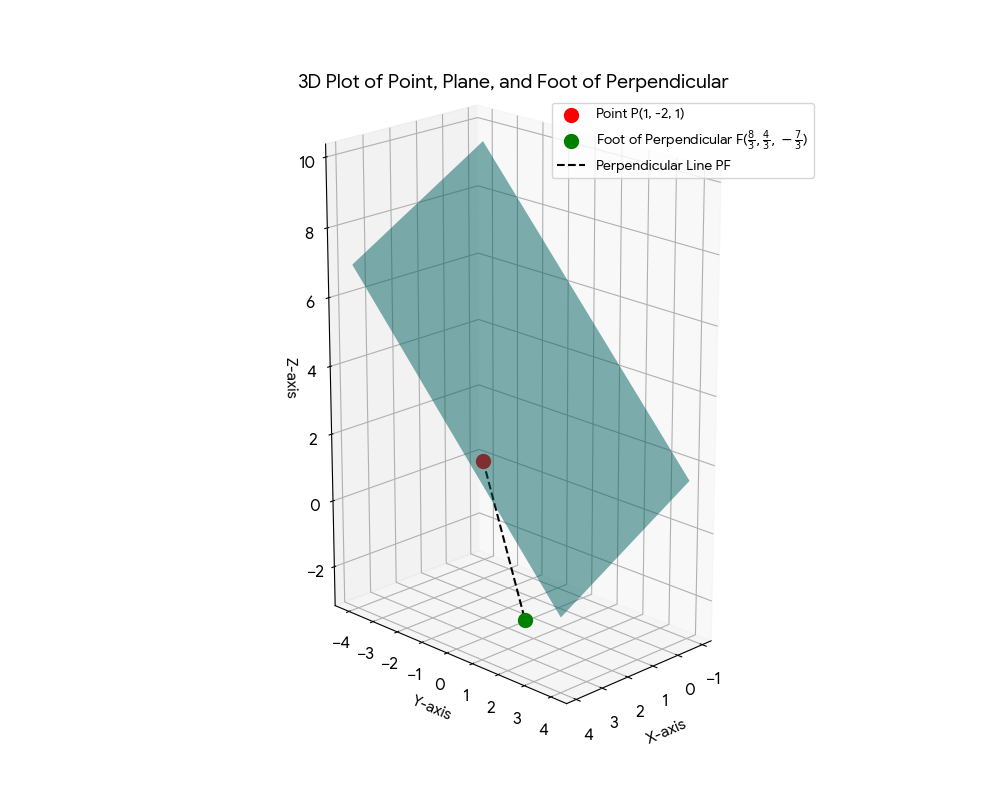
\includegraphics[width=\columnwidth, height=0.8\textheight, keepaspectratio]{figs/python_plot.png}     
\end{frame}


\end{document}